% !Mode:: "TeX:UTF-8"
	\title{第一次上机实验报告:数据探索}
	\author{江昱峰 21009200038} 
\documentclass {article}
\usepackage[UTF8]{ctex}
\usepackage{graphicx}
\usepackage{float}
\usepackage{hyperref}
\usepackage{makecell}
\begin{document}
%\begin{sloppypar}
\maketitle{}
\section{背景介绍}
	当今时代,是有着海量数据且每天仍在涌现大量数据的大数据时代。而对于生物学来说,生物体内的细胞、基因、基因表达产物等本身就是数量极为庞大的群体,更需要用科学专业的数据挖掘算法和模型来完成数据采集获取、数据存储、数据处理、数据分析、数据可视化等的步骤过程。
	
\section{实验目的}
	\begin{itemize}
		\item 实践生物学数据挖掘的数据采集获取、数据存储、数据处理(数据清洗过滤、归一化等)、数据分析、数据可视化等的步骤过程,从而对数据挖掘和数据探索有更深的认识和掌握;
		\item 掌握单细胞RNA-seq测序数据集的读取、AnnData对象的处理、基因表达数据矩阵中“0”的含义与处理方案等生物学领域的数据挖掘知识和技术;
		\item 掌握Python中ndarray、Series、DataFrame等数据类型的构成与常用操作;
		\item 掌握Python中数据分析相关的numpy、pandas、scipy、sklearn、matplotlib、seaborn等库中常用函数的使用;
		\item 掌握常见统计量和相关系数、相似/异度计算方法的意义与计算公式;
		\item 掌握用Cytoscape等软件绘制网络关系图;
		\item 加深对算法模型的时间复杂度与创建数组矩阵等的空间复杂度的平衡、优化的认识。
	\end{itemize}	

\section{任务描述}
	\subsection{数据的汇总统计分析}
		\begin{itemize}
			\item 针对单个细胞(样本),基因表达的取值范围;
			\item 数据矩阵中“0”的出现及其含义,给出统计分析结果,并据此给出处理的方案;
			\item 给出均值、方差等的统计分析结果。
		\end{itemize}

	\subsection{数据的可视化}
		\begin{itemize}
			\item 针对上述统计分析给出其可视化结果;
			\item 针对以上统计分析及可视化结果给出分析和总结。
		\end{itemize}

	\subsubsection{构建共表达网络并可视化}	
		\begin{itemize}
			\item 通过计算任意两个基因对之间的皮尔森相关稀疏,构建基因之间的共表达网络,并 
			进行分析; 
			\item 通过计算细胞之间的相似性,构建细胞之间的相似性网络,并进行分析。
		\end{itemize}
	
		注:
		\begin{itemize}
			\item 网络可视化可以采用 cytoscape,但是不限于此工具。 
			\item 数据可视化可以采用任何熟悉的编程工具或者软件。
		\end{itemize}
	
\section{数据描述}
	实验先后提供了三组数据集,但按照老师和助教修改后的要求,本实验只基于其中的Breast\_Cancer\_3p\_filtered\_feature\_bc\_matrix数据集进行挖掘分析。下面是对于三组数据集单细胞RNA-seq测序数据的描述:
	\subsection{Visium\_Human\_Breast\_Cancer\_filtered\_feature\ \\ bc\_matrix.tar.gz和Breast\_Cancer\_3p\_filtered\_ \\ feature\_bc\_matrix}
		下载自 10× Genomics 的浸润性导管癌乳腺组织的 RNA-seq 数据。Barcodes.tsv.gz 
		主要包含细胞信息。features.tsv.gz 包含基因信息。matrix.mtx.gz 为基因表达矩阵, 
		行表示细胞,列表示基因,其中的值为特定基因在特定细胞中的表达值。 
		
		Scanpy 中的 read\_10x\_mtx( )函数可以直接将数据集读取为 AnnData 对象,以便后 
		续分析。 
		
		其中AnnData数据类型的构成和属性如下图所示:
		\label{构成和属性}
		\begin{figure}[H]
			\centering
			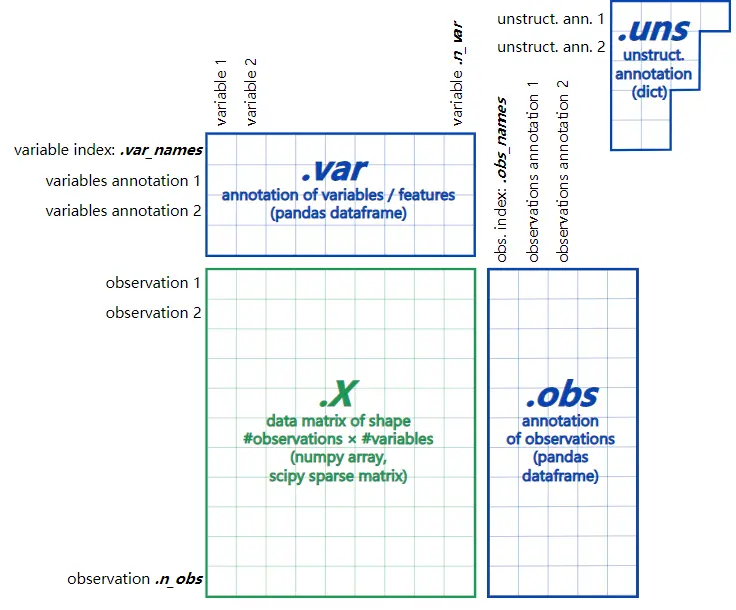
\includegraphics[width=4.5in,height=3in]{figures/fig1.png}
			\caption{AnnData数据类型的构成和属性}
		\end{figure}
	
		这些属性各自的功能和数据类型如下表所示:
		\begin{table}[H]
			\caption{AnnData属性的功能和数据类型}
			\centering
			\begin{tabular}{ccc}
				\hline
				属性名称      & 功能         & 数据类型                                               \\ \hline
				adata.X   & 矩阵数据       & numpy, scipy sparse, matrix \\ 
				adata.obs & 观察值数据      & pandas dataframe                                   \\ 
				adata.var & 特征和高可变基因数据 & pandas dataframe                                   \\ 
				adata.uns & 非结构化数据     & dict                                               \\ \hline
			\end{tabular}
		\end{table}
	
		其中,adata.X在本实验中的具体数据类型为scipy.sparse.\_csr.csr\_matrix,这是一种稀疏矩阵,主要有以下三种属性:
		\begin{table}[H]
			\caption{scipy.sparse.\_csr.csr\_matrix属性的功能和数据类型}
			\centering
			\begin{tabular}{ccc}
				\hline
				属性名称        & 功能              & 数据类型    \\ \hline
				mtx.indptr  & 每行对应于下面两种属性内的索引 & ndarray \\ 
				mtx.indices & 每行内非0元素的列索引     & ndarray \\ 
				mtx.data    & 所有非0元素的值        & ndarray \\ \hline
			\end{tabular}
		\end{table}
	
		具体的,mtx中第i行的列下标存储在indices[indptr[i]:indptr[i+1]],并且它们对应的值存储在data[indptr[i]:indptr[i+1]]。如果没有提供shape参数,那么矩阵的维数就会根据index arrays自动推断。
	
	\subsection{GSE212890 数据集}
		来自47名癌症患者包括肿瘤和正常组织的肿瘤浸润NK细胞,包括‘THCA’, ‘FTC’, 
		‘RC’, ‘BRCA’, ‘PACA’, ‘OV’, ‘UCEC’, ‘ESCA‘八种癌症;包含 11963 个细胞, 28991 个 
		基因(6044 个正常细胞,5019 个肿瘤细胞)。 
		
		NK\_rawcount.barcodes 数据包含两列,第一列是 index,第二列为细胞的标识 
		(cellID),用来标记不同的细胞。 
		
		NK\_rawcount.genes:数据包含两列,第一列是 index,第二列为基因的别名 
		(gene\_alias,与 gene symbol 的区别自行搜索,此处不过多赘述),用来标记不同 
		的基因。 
		
		NK\_rawcount.mtx:细胞中基因表达量的稀疏矩阵。第一行三个数值分别表示: 
		细胞总数,基因总数和基因表达总量。包含三列,其中第一列数值 i 表示第 i 个细 
		胞,第二列数值 j 表示第 j 个基因,第三列数值 m 表示第 i 个细胞中,基因 j 的表达 
		量为 m。 
		
		注意:在 NK\_rawcount.barcodes 与 NK\_rawcount.genes 中 index 是从 0 开始 
		的,而在 NK\_rawcount.mtx 中均从 1 开始,需要注意对应关系。
		 
		GSE212890\_NK\_metadata.csv:该文件记录数据的一些其他信息,其中 cellID 与 
		NK\_rawcount.barcodes 文件 中 的 cellID 对应 ;meta\_histology 为肿 瘤类型 ; 
		meta\_tissue 标记该细胞是肿瘤细胞还是正常细胞;Majortype 为该细胞的主要类型。 
		以上数据解压后可在 PyCharm 上直接进行预览或者用 excel 预览(除 csv 文件 
		外不推荐 excel),数据读取和处理可参考 Scanpy 文档。
		
		此数据集的数据类型也为AnnData,具体的构成和属性见\hyperref[构成和属性]{上一部分}。
	
\section{实验原理}
	实验中涉及的一些统计量的含义、意义和计算公式如下:
	\label{实验原理}	
	\begin{table}[H]
		\centering
		\caption{实验中统计量的意义和计算公式}
		\begin{tabular}{ccl}
			\hline
			统计量 & 意义(度量数据) & 计算公式                                                                                                                                                                                                                                                                                                                                                                                                                                                                                                                                                                                                                                                                                                                                                                                                                                                                                                                                                                                                                                                                          \\ \hline
			方差  & 偏离程度               & $S^2=\frac{1}{n-1} \sum_{i=1}^n\left(X_i-\bar{X}\right)^2$  \\ \hline
			偏度  & 不对称性               & \makecell[l]{$Skew(X)=E\left[\left(\frac{X-\mu}{\sigma}\right)^3\right]$ \\ 或$\frac{EX^3-3 \mu \sigma^2-\mu^3}{\sigma^3}$} \\ \hline

			峰度  & 陡峭程度               & \makecell[l]{$Kurtosis=$ \\ $\frac{1}{n-1} \sum_{i=1}^n\left(x_i-\bar{x}\right)^4 / S D^4-3$} \\ \hline
			皮尔森相关系数 & 线性相关程度 & \makecell[l]{$r=\frac{l_{xy}}{\sqrt{l_{xx}l_{yy}}}=$ \\  $\frac{\sum_{i=1}^{n}{(x-\tilde{x})(y-\tilde{y})/(n-1)}}{\sqrt{\sum_{i=1}^{n}{(x-\bar{x})^{2}/(n-1)}}\cdot\sqrt{\sum_{i=1}^{n}{(y-\bar{y})^{2}/(n-1)}}}$}  \\
			\hline 
		\end{tabular}
	\end{table}
				
%				
\section{实验环境}
本次实验的实验环境见下表:
	\begin{table}[H]
		\caption{实验环境}
		\centering
		\begin{tabular}{cc}
			\hline
			类型 & 工具配置 \\ \hline
			操作系统 & AWS(亚马逊云)服务器- Linux(Ubuntu 20.04)  \\
			编程语言 & Python 3.10(Anaconda 2023 - Jupyter Notebook) \\ 
			编译器  & VScode                                      \\ 
			软件   & Cytoscape                                     \\ \hline
		\end{tabular}
	\end{table}
		
\section{分析步骤}
	先进行数据读取。我用scanpy库中的read\_10x\_mtx函数对单细胞数据集进行读取,得到AnnData对象。然后,我获取这两者的X属性,得到scipy.sparse.\_csr.csr\_matrix对象,即数据集中的mtx文件。接下来,我将分别根据不同任务进行计算分析。
	
	紧接着是数据预处理。首先,经检查,数据中无缺失值、重复值、异常值(离群值等)等。接着,我进行了数据过滤:先是基本过滤,考虑到数据集中有很多表达基因数很少的细胞,以及在很少的细胞中表达的基因,第二步我对上一步得到的scipy.sparse.\_csr.csr\_matrix对象进行了数据过滤,去除掉了表达基因3000以下的细胞和在50个细胞以下表达的基因,得到14797个细胞和2728个基因;基本过滤之后我又进行了去除表达过多线粒体基因和总计数过多的细胞、对对象进行切片等较为高级的过滤。然后,我进行了一些数学运算,将总计数归一化(库大小校正)为每单元格 10,000 个读取以便计数在单元格之间具有可比性,对数据进行对数化,并将每个基因缩放到单位方差(剪辑值超过标准偏差10)。
	
	然后,我根据实验任务进行了具体的数据挖掘分析,步骤如下。
	
	\subsection{数据的汇总统计分析}
		\subsubsection{单个细胞(样本)基因表达的取值范围}
			要计算单个细胞(样本)基因表达的取值范围,主要需要获取细胞(样本)所有基因表达量总和的最大值和最小值。我通过遍历scipy.sparse.\_csr.csr\_ \\ matrix对象的indptr属性来遍历数据集中的所有细胞,根据每个细胞indptr属性的前后索引,将其对应的data属性,即基因表达量区间内的值求和,从而分别计算每个细胞基因表达量的总和,并筛选出最大值和最小值,最终得到单个细胞(样本)基因表达的取值范围。
		
		\subsubsection{数据矩阵中“0”的出现与含义,统计结果与处理方案}
			数据矩阵中“0”的出现通常表示该细胞在该基因上的基因表达值为0,意味着该基因在该细胞中没有被检测到或者表达水平非常低。不过需要注意的是,0并不一定表示基因在该细胞中完全没有表达。在单细胞转录组数据中,基因表达计数通常具有一定的噪音和技术误差。因此,对于非常低的表达水平,可能会被测量为0,但实际上可能存在微弱的基因表达。这也是为什么在单细胞转录组数据分析中,需要进行适当的数据预处理和归一化来处理这种噪音和技术误差。
		
			对于数据矩阵中“0”的统计,由于数值已经固定为0,计算基因表达量相关的统计量,如最值、总和、均值等没有很实际的意义。不过,我们可以计算所有细胞以及每个细胞、基因中“0”出现的次数、比例等数据类型,每类数据又还可以分别计算最值、求和、均值等统计量。
		
			据此,我提出了高效便捷的处理方案,见\hyperref[处理方案]{8.1.2}部分。
		
		\subsubsection{均值、方差等的统计分析结果}
			我分别从细胞、基因作为主体对象这角度,计算了数据集的统计量。除了实验任务中给出的均值、方差(依照课本,这里我选取无偏估计的样本方差$S^2$)之外,我还计算了最值、极差、中位数、四分位数、总和、偏度、峰度等统计量,其中方差、偏度和峰度的计算公式见\hyperref[实验原理]{实验原理}部分。
		
	\subsection{数据的可视化}
		\subsubsection{可视化结果}
			针对上述统计分析结果,我通过绘制小提琴图,将结果进行可视化。小提琴图将箱线图和核密度图结合并吸取了二者的优点,可以同时展示中位数、四分位数、最值等统计量和数据整体在不同区间的分布频率。除此之外,我还计算并可视化了高度可变基因的表达情况、所有细胞中表达占比最高的基因等。
		
		\subsubsection{分析和总结}
			见\hyperref[分析和总结]{9.2.1}部分。
		
	\subsection{构建共表达网络并可视化}
		\subsubsection{基因对之间的皮尔森相关系数与共表达网络}
			\label{基因对之间皮尔森相关系数与共表达网络}
			基因对之间的相关性,具体指基因在所有细胞中基因表达量数组之间的相关性。我先将scipy.sparse.\_csr.csr\_matrix矩阵从稀疏矩阵转换为稠密矩阵,从而得到行为细胞,列为基因,值为基因表达量的二维矩阵。然后,我根据皮尔逊相关系数公式,计算出所有基因对两两之间的皮尔森相关系数。接着,为了使共表达网络中基因对之间的相关性足够充分、剔除掉相关性不够强的基因对关系从而降噪,我根据皮尔森相关系数大小与相关性强弱的关系(见下表),筛选出相关系数达到0.9、相关性较强的基因对,并利用Cytoscape软件构建出基因之间的共表达网络。
			\begin{table}[H]
				\centering
				\caption{皮尔森相关系数大小与相关性强弱的对应关系} 
				\begin{tabular}{cccccc}
					\hline
					取值范围 & 0.0\~{}0.2 & 0.2\~{}0.4 & 0.4\~{}0.6 & 0.6\~{}0.8 & 0.8\~{}1.0 \\
					相关性强弱 & 极弱/无相关 & 弱相关 & 中等程度相关 & 强相关 & 极强相关 \\
					\hline
				\end{tabular}
			\end{table}
		
		\subsubsection{细胞之间的相似性与相似性网络}
			细胞之间的相似性,具体和\hyperref[基因对之间皮尔森相关系数与共表达网络]{上一部分}中类似,指的是基因表达量的相似性。而对于度量和计算细胞的基因表达量之间的相似性,有很多方法和相关变量,主要分为相似度和相异度两大类。其中相似度相关的方式主要有(广义)Jaccard系数、余弦相似度等;相异度则主要通过距离度量,常见的度量方式除了教材和课件中给出的欧式距离、闵可夫斯基距离、马氏距离之外,还有曼哈顿距离等等。这些度量方式都有各自适合的条件和情况,而对于细胞基因表达这一类高维且稀疏的数据,余弦相似度这一计算方式最为适合。因为它可以忽略向量的大小差异,而只关注它们的方向相似性,适用于处理稀疏的数据,这在基因表达数据中非常有用。
			
			因此,我先用余弦相似度计算出细胞之间的相似性,然后根据余弦相似度的定义,筛选出余弦相似度达到0.95,即向量夹角不超过$ \arccos{0.95}=18.195^{\circ}$的细胞对,并利用Cytoscape软件构建出细胞之间的相似性网络。
		
\section{实验结果及可视化}
	\subsection{数据的汇总统计分析}
		\subsubsection{单个细胞(样本)基因表达的取值范围}
			基因表达的取值范围为34.657\~{}18506.270。
			\subsubsection{数据矩阵中“0”的出现与含义,统计结果与处理方案}
			关于0的统计结果:
			\begin{table}[H]
				\centering
				\caption{数据矩阵中“0”相关的统计结果} 
				\begin{tabular}{cc}
					\hline
					统计指标 & 数值 \\ \hline
					0出现总次数            & 25815867 \\                                                         
					0出现比例             & 63.954\%  \\
					细胞中0出现次数均值/基因总数 & 1744.669/2728  \\
					基因中0出现次数均值/细胞总数 & 9463.294/14797	 \\ 
					\hline
				\end{tabular}
			\end{table}
		
			\label{处理方案}
			关于0的处理方案:直接利用获取的scipy.sparse.\_csr.csr\_matrix这一稀疏矩阵数据类型进行操作,而不是先通过todense函数进一步转化为稠密矩阵然后再继续操作。这样做有诸多优势:时间方面,虽然理论的时间复杂度没有本质的提升,但由于稀疏矩阵中非0值占比只有约40\%,因此处理速度能够变快2倍左右,缩短了程序的运行时间;空间方面,可以节省约60\%的空间开销,充分节省了计算机硬件的存储空间资源,工业应用中可能还可以降低成本。
		
		\subsubsection{均值、方差等的统计分析结果}
			数据集分别按细胞、基因作为统计主体的统计分析结果如下表所示:
			\begin{table}[H]
				\centering
				\caption{统计分析结果}
				\begin{tabular}{ccc}
					\hline
					主体    & 细胞            & 基因  \\
					\hline
					均值    & 584.530     & 3170.583       \\
					方差    & 1169331.552 & 75288.716 \\
					最大值   & 15256.408        & 170288       \\
					最小值  4113.165          & 1951.434       \\
					极差    & 232.410        & 2161.731        \\
					中位数   &  1049        & 3179.337            \\
					上四分位数 & 604.462         & 3351.685 \\
					下四分位数 & 74.410          & 2999.724 \\
					偏度    & 4.891         & -0.290 \\
					峰度    & 33.772         & 0.620 \\
					\hline                            
				\end{tabular}
			\end{table}
	
	\subsection{数据的可视化}
		\subsubsection{可视化结果}
			数据集分别按细胞、基因作为主体绘制的小提琴图如下所示:
			\begin{figure}[H]
				\centering
				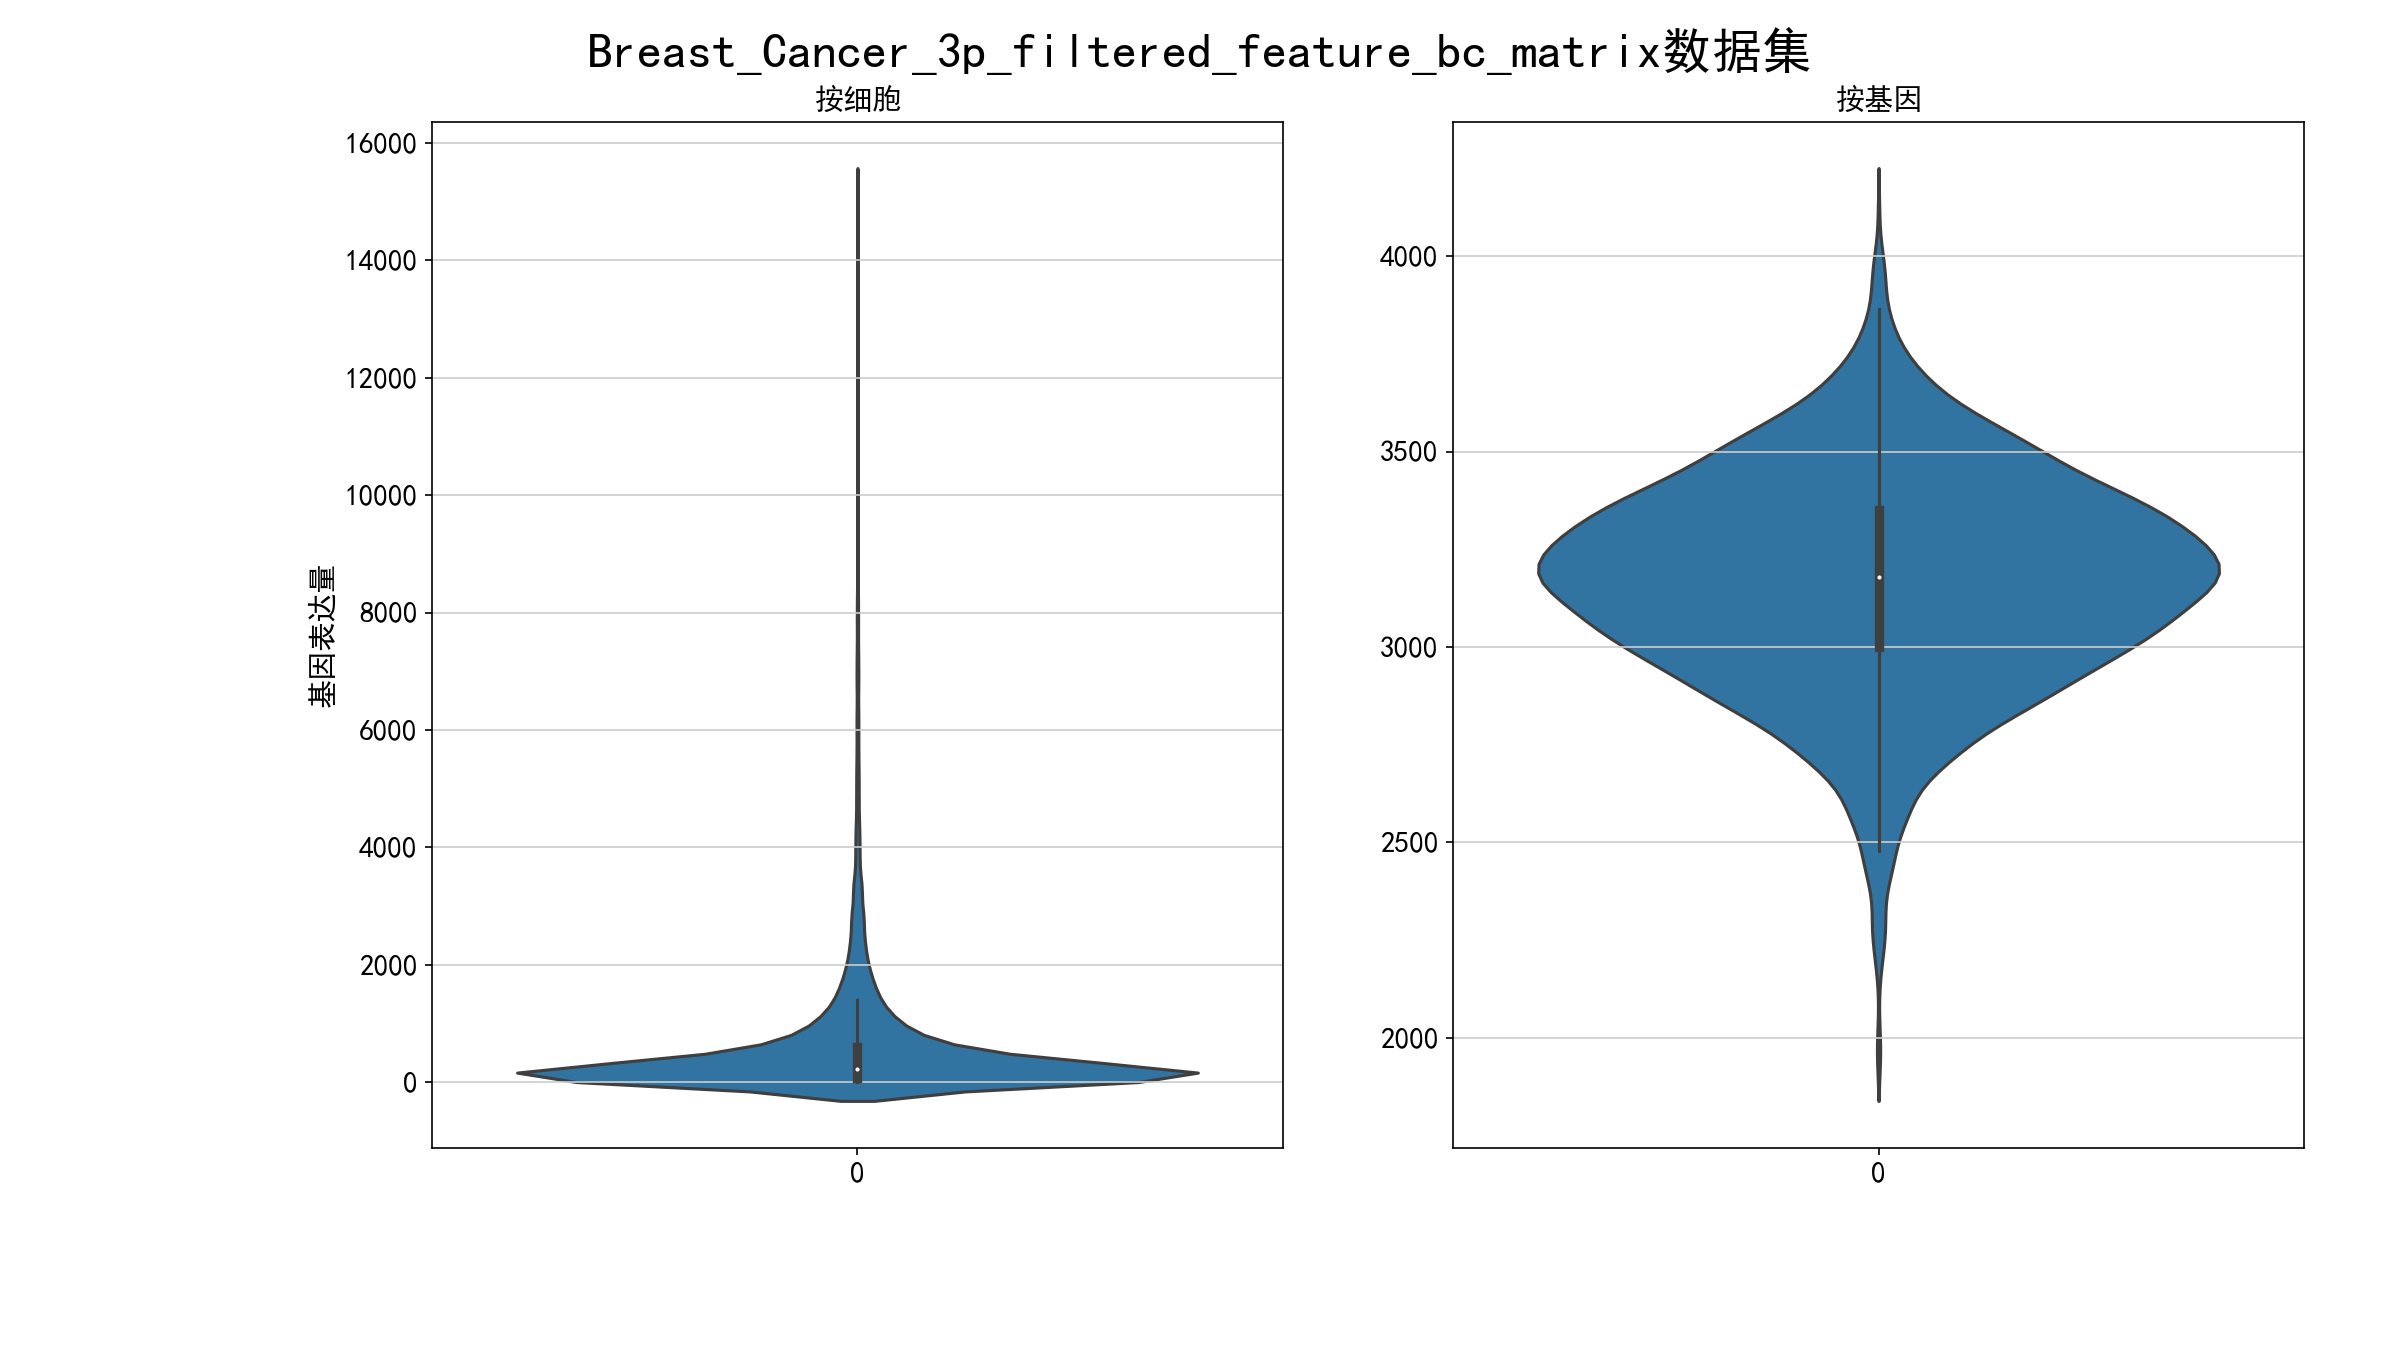
\includegraphics[width=4.5in]{figures/fig2.png}
				\caption{统计分析的可视化结果(小提琴图)}
			\end{figure}

			高度可变基因的表达情况如下图所示:
			\begin{figure}[H]
				\centering
				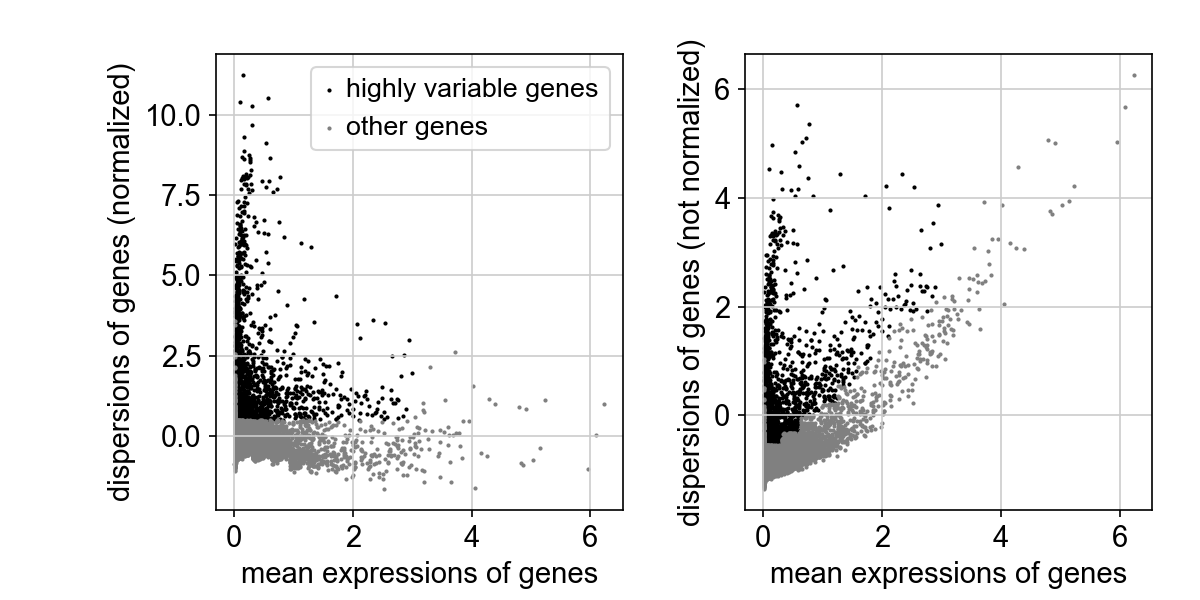
\includegraphics[width=4.5in]{figures/fig3.png}
				\caption{高度可变基因表达情况散点图}
			\end{figure}
			
			所有细胞中表达占比最高的基因如下图所示:
			\begin{figure}[H]
				\centering
				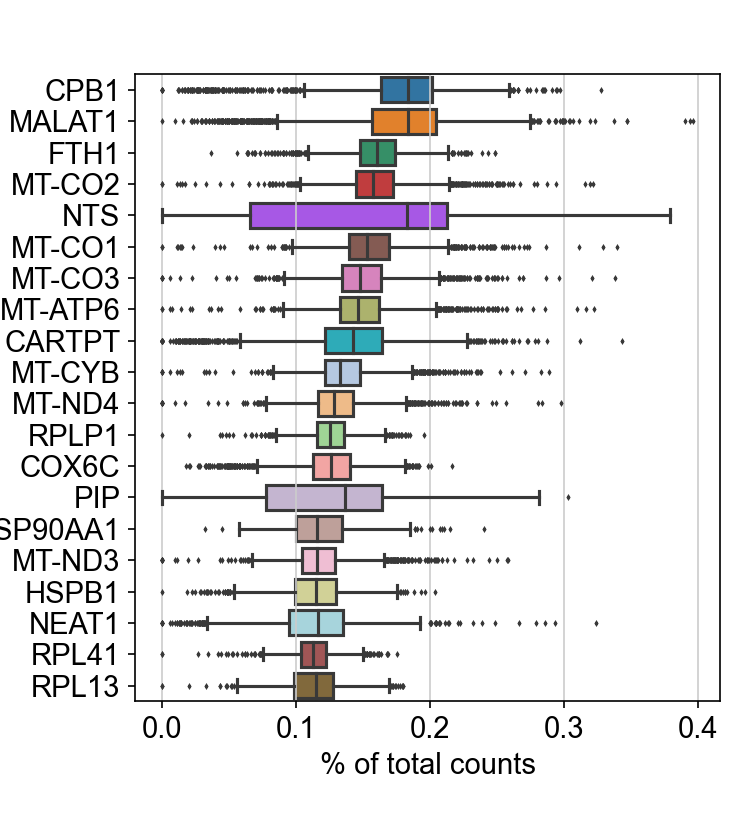
\includegraphics[width=3.5in]{figures/fig4.png}
				\caption{所有细胞中表达占比最高的基因}
			\end{figure}
			
		\subsubsection{分析和总结}
			见\hyperref[分析和总结]{结果分析与探讨部分中对应内容}。
		
	\subsection{构建共表达网络并可视化}
		\subsubsection{基因对之间的皮尔森相关系数与共表达网络}
			基因对两两之间的皮尔森相关系数结果数据规模较大,本文不方便展示,因此我放在了提交材料的结果目录中,详见对应Excel表格;共表达网络如下图所示:
				\begin{figure}[H]
					\centering
					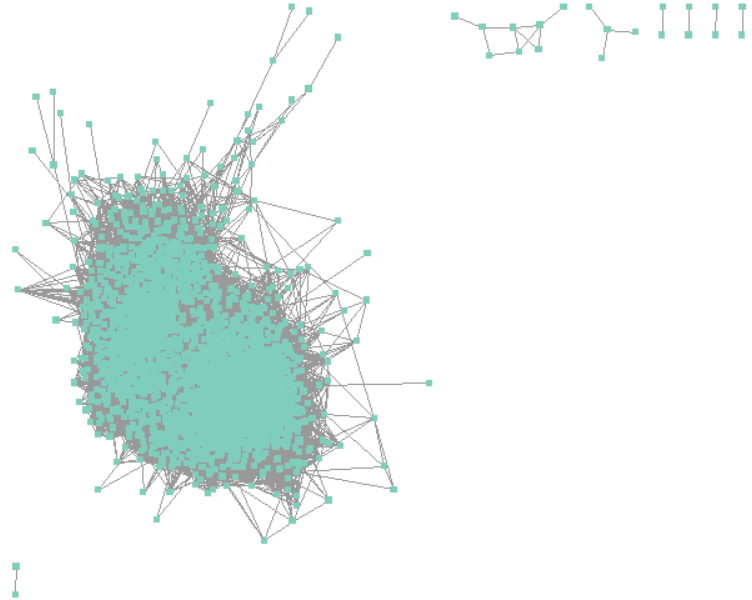
\includegraphics[width=4.5in,height=4.5in]{figures/fig5.jpg}
					\caption{基因之间的共表达网络}
				\end{figure}			
		
		\subsubsection{细胞之间的相似性与相似性网络}
			细胞两两之间的相似度规模同样较大,因此也放在了提交材料的结果目录中,详见对应Excel表格;相似性网络如下所示:
				\begin{figure}[H]
					\centering
					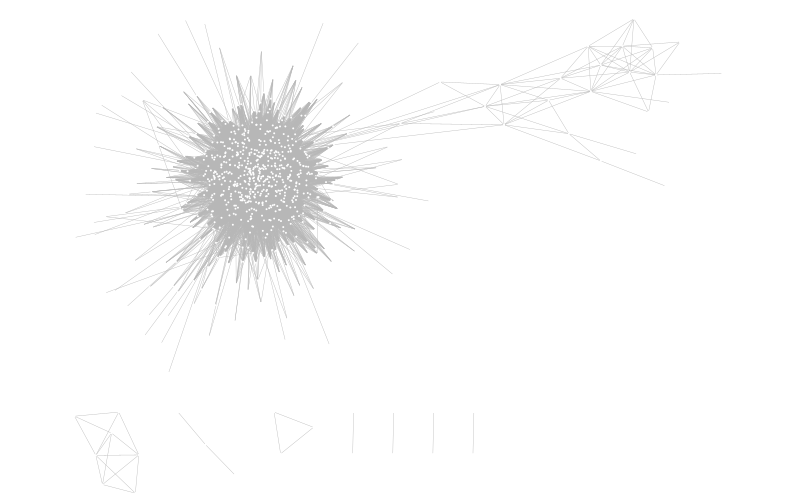
\includegraphics[width=4.5in,height=4in]{figures/fig6.png}
					\caption{细胞之间的相似性网络}
				\end{figure}			
		
\section{结果分析}
	\subsection{数据的汇总统计分析}
		\subsubsection{单个细胞(样本)基因表达的取值范围}
			单个细胞(样本)基因表达的取值范围果对于后续数据挖掘有以下几点影响和启示:
			\begin{itemize}
				\item 可以反映和检查数据过滤步骤是否成功、正确;
				\item 可以对数据的规模有大致的了解和把握;
				\item 可用于在数据预处理步骤中对数据进行进一步的归一化、标准化和数据归约等操作。
			\end{itemize}
		
		\subsubsection{数据矩阵中“0”的出现与含义,统计结果与处理方案}
			数据矩阵中“0”的出现与含义、统计结果与处理方案对于后续数据挖掘有以下几点影响和启示:
			\begin{itemize}
				\item 可以反映和检查基因表达情况是否合理;
				\item 可以对细胞中不同基因和基因在不同细胞中的表达活跃程度有大致的了解和把握;
				\item 可以通过稀疏矩阵数据结构的存储来缩短程序的运行时间、节省计算机硬件的存储空间资源,从而相应地提高效率、降低成本。
			\end{itemize}			
		
		\subsubsection{均值、方差等的统计分析结果}
			均值、方差等的统计分析结果对于后续数据挖掘有以下几点影响和启示:
			\begin{itemize}
				\item 可以反映和定性地检查数据的计算结果大体是否正确;
				\item 可以对数据的集中和离散分布特征有大致的了解和把握。
			\end{itemize}

	\subsection{数据的可视化}
		\subsubsection{可视化结果}
			可视化结果对于后续数据挖掘有以下几点影响和启示:
			\begin{itemize}
				\item 可以展示数据的总体分布情况;
				\item 可以展示各部分区间的大致比例。
			\end{itemize}
			
		\subsubsection{分析和总结}
			\label{分析和总结}
			针对以上统计分析及可视化结果,可以得出以下几点分析和总结:
			\begin{itemize}
				\item 数据集中无论是同一细胞中所有基因表达的比例,还是同一基因在所有细胞中表达的比例普遍都很少,只有5\%到10\%左右,这与生物学知识相符。
				\item 按基因作为主体的基因表达总量分布相对较分散。
			\end{itemize}
		
	\subsection{构建共表达网络并可视化}
		\subsubsection{基因对之间的皮尔森相关系数与共表达网络}
			基因对之间皮尔森相关系数与共表达网络反映了基因之间的相关性强弱,以及相关性较强的基因对占所有基因对的比例,同时对于后续数据挖掘有以下几点影响和启示:
			\begin{itemize}
				\item 可以展示基因对之间的相关性强弱并可视化出网络关系图;
				\item 可以进一步筛选出相关性较强的基因并可视化。
			\end{itemize}

		\subsubsection{细胞之间的相似性与相似性网络}
			细胞之间相似性与相似性网络类似上一部分,反映了细胞之间的相似性大小,以及相似性较大的细胞对占所有细胞对的比例,同时对于后续数据挖掘有以下几点影响和启示与上一部分类似:
			\begin{itemize}
				\item 可以展示细胞之间的相似性大小并可视化出网络关系图;
				\item 可以进一步筛选出较为相似的基因并可视化。
			\end{itemize}			

\section{实验讨论}
	\subsection{优缺点分析}
		本次实验过程有以下几点优点:
		\begin{itemize}
			\item 在数据分析前和绘制关系图前都进行了数据过滤、降噪,提高了数据质量和纯度;
			\item 使用稀疏矩阵存储数据,缩短程序的运行时间、节省计算机硬件的存储空间资源,从而相应地提高效率、降低成本;
			\item 使用的算法模型符合应用条件情况,计算结果符合科学知识,具有合理性;
			\item 使用的模型算法稳定,结果具有鲁棒性、可扩展性。
		\end{itemize}
		
		不过,实验也存在一些缺点,如网络关系图的优化等等。
		
	\subsection{改进方法}
		本次实验有以下几点可以进一步改进的方法:
		\begin{itemize}
			\item 算法模型的空间复杂度还可以进一步优化;
			\item 网络关系图还可以进一步美化。
		\end{itemize}
		
\section{心得体会}
	做完本次实验,除了掌握了实验目的部分中所有内容的收获之外,我还有以下几点心得体会:
	\begin{itemize}
		\item 数据挖掘大体按照数据采集获取、数据存储、数据I/O、数据处理(数据清洗,如剔除缺失值、重复值、异常值等等;数据预处理,如数据类型转换,数据归一化、标准化、离散化等等;数据降噪/平滑化;数据归约,如维度、属性、特征归约,数据采样等等;特征提取)、数据分析、数据可视化的步骤过程进行;
		\item 数据挖掘前需要先对数据的规模、特征有大致的了解和把握;
		\item 编程前要先对算法的时间复杂度和创建矩阵数组等变量的空间复杂度尽可能地取得平衡和优化,同时及时释放内存,防止出现运行时间过长、内存不足,甚至对计算机造成损坏等情况。
	\end{itemize}

\section{参考文献}
	[1] 白墨,《scanpy 单细胞分析包图文详解 01 | 深入理解 AnnData 数据结构》,2021,https://zhuanlan.zhihu.com/p/369705199

%\end{sloppypar}
\end{document}
\endinput